\documentclass[a4paper]{article}
\usepackage{a4wide}
\usepackage[french]{babel}
\usepackage{fancyhdr, graphicx}
% Voir https://stackoverflow.com/questions/544907/remove-boxes-from-hyperlinked-toc-in-latex
\usepackage[hidelinks]{hyperref}
%
\usepackage[utf8]{inputenc}
\usepackage{xspace}
\let\OldTexttrademark\texttrademark
\renewcommand{\texttrademark}{\OldTexttrademark\xspace}%
\renewcommand{\headrulewidth}{0pt}
\fancyhead[R]{}
\fancyhead[L]{

\includegraphics[width=1.5cm]{logo_chainons_noirs.png}
}
\fancyhead[C]{

\includegraphics[width=6.5cm]{logo_sesame_noir.png}
}
%\hypersetup{%
%    pdfborder = {0 0 0}
%}
\newcommand{\version}{\vspace{10pt}\\ Version 1.0}
\newcommand{\smallvspace}{\vspace{4pt} \\}
\begin{document}
\title{Livre blanc \vspace{10pt} \\
\large la Certification LCB-FT* en 3 clics~\footnote{Lutte contre le blanchiment des capitaux et le financement du terrorisme}}
\author{Cyril Chad\'e, Thomas Guerber and Christophe Ramananjaona}
\date{\today\version}
\maketitle
\thispagestyle{fancy}
\tableofcontents
\newpage
\section{Introduction}

La technologie de la blockchain est adoptée par un nombre croissant d’industries, et les actifs crypto sont devenus un élément permanent du système financier. Ils intègrent aussi les économies de l’entertainment, de l’art, de l’assurance, du jeux, de la distribution, de la logistique, de l’immobilier et le besoin initial de sécurité et de conformité légale évolue en une pression régulatoire de plus en plus forte. 
Néanmoins par définition, sur les écosystèmes blockchains on ne sait pas avec qui on interagit, puisque cette technologie repose sur des registres distribués, la cryptographie et le pseudonymat. D’autre part, la régulation est encore souvent totalement inadéquate et les autorités législatives se méfient surtout des activités de blanchiment d’argent et de financement du terrorisme. En effet, celles-ci pourraient encore représenter des milliards de dollars de transactions illicites.
La majeure partie de l’industrie crypto s’accorde maintenant sur le besoin de plus de conformité, de transparence, et de légalité, notamment pour permettre l’adoption de masse, et pour accueillir des milliards de nouveaux utilisateurs. Par conséquent, la traçabilité des fonds devient une question fondamentale pour les régulateurs ainsi que pour les entreprises et les particuliers. \\

Nous pouvons y parvenir en intégrant une couche analyse on-chain des transactions, baptisé “KYT” ou "Know Your Transaction" (en miroir du “KYC” de la TraFi : Finance Traditionnelle), dans un smart contract qui maintiendra le portefeuille des utilisateurs dans un espace sûr et digne de confiance. \\

Notre objectif est de créer progressivement des zones de confiance où les transactions financières entre les portefeuilles certifiés et les smart contracts certifiés sont considérées comme conformes. Ainsi, la communauté Web3 disposera d'un écosystème sûr et sécurisé pour développer son économie, tout en conservant l'esprit de protection de la vie privée et de décentralisation qui est attaché à ses racines. \\

Tout comme le pseudonymat est un fondement même de la technologie de la blockchain, par définition, le pendant structurel est que toutes les transactions peuvent être retracées, tous les blocs peuvent être lus, tous les portefeuilles peuvent être vérifiés. Notre objectif est de donner progressivement un accès universel à ces outils d’historique complet des transactions, de telle sorte que n’importe quel portefeuille puisse-t’être certifié comme étant conforme, interagir avec ses pairs et puisse mettre de côté les autres portefeuilles qui eux ne le seraient pas. Notre communauté de bâtisseurs du Web3 est prête désormais à créer un écosystème économique sûr et sécurisé, dans une industrie libre et protégeant la vie privée. \\

Les législateurs, sans étouffer l’innovation, veulent garder le contrôle sur les business crypto, et par-dessus tout, s’assurer qu’il ne s’agisse pas d’un passe-partout pour blanchir des fonds illégaux, du crime, des fraudes en ligne ou des rançongiciels. Les entreprises, les ONG, les entrepreneurs, les fondations, les investisseurs, et chaque individu de même, veulent travailler, progresser, et créer de la valeur dans un environnement respectueux des droits humains et dédié à la croissance et à l'épanouissement de la société. \\

La Blockchain contribue à ces valeurs, renforçant la vie privée, la sécurité des interactions, et un accès neutre et universel.

\subsection{L’entreprise Sesame}
Sesame.fi est basée en France, et spécialisée dans la certification de la conformité crypto. Nous voulons construire le prochain standard global de conformité pour le Web3 et accélérer son adoption par des entités régulées et des individus ayant besoin de transparence. \\

Le coeur de notre service est une procédure facile d’utilisation, basée sur un score de conformité aux critères de Lutte contre le blanchiment d'argent et de financement du terrorisme (LCB-FT) ou plus précisément de KYT (Know Your Transaction), connaitre l’historique de la transaction. Ce service assurera la certification de portefeuilles et de leurs propriétaires et les conduira vers des espaces de confiance Web3, où tous leurs pairs pourront échanger en toute sécurité, sans crainte d'être contaminés par des activités frauduleuses ou suspicieuses. \\

Grâce aux partenaires fournissant les standards mondiaux des plus élevés, grâce aux équipes d’experts Web3 et grâce aux partenariats produits, nous réalisons l’un des besoins les plus attendus, la transparence dans l’industrie.
\subsection{L’équipe}
En tant que Startup fintech française, nous rassemblons une équipe d’experts solides et complémentaires de domaines et d’industries variées, tous impliqués dans la blockchain et le Web3 depuis plusieurs années, pour réussir ce nouveau projet entrepreneurial.

\begin{itemize}
\item 
Christophe Ramananjaona \smallvspace
Géophysicien (PhD), développeur en calcul haute-performance, avec plus de 20 ans d’expertise dans le traitement des données et des modèles numériques, pour la recherche universitaire, l’industrie pétrolière et gazière, et un vif intérêt pour les smart contrats et l’exploitation de la technologie de la blockchain.

\item 
Cyril Chadé \smallvspace
Entrepreneur, investisseur et conseiller de gouvernements, a créé 4 entreprises dans le Web1, Web2 \& Web3, dont 2 ont été vendues avec succès et existent encore. Il a conseillé des gouvernements européens, des Ministres, des législateurs et des institutions publiques, ainsi que de nombreuses compagnies technologiques comme Facebook, Lime, Google.

\item 
Thomas Guerber \smallvspace
Investisseur Crypto depuis 2012, juriste et financier d’entreprise, mais avant celà journaliste, copywriter, et créateur dans l’espace blockchain. Thomas est également certifié AMF, (Autorité des Marchés Financiers).
\end{itemize}

\subsection{Les problèmes}
Alors que la blockchain et les actifs numériques commence à être largement adoptés et régulés, les banques, les institutions financières mais aussi les marques de luxe, les artistes, les maisons d’enchère, les acteurs de l’immobilier, les chercheurs, les logisticiens, et d’autres encore, souhaitent entrer dans le monde décentralisé avec autant de garanties que possible, pour: 

\begin{itemize}
\item Acheter et vendre des actifs numériques
\item Répondre aux besoins de leurs clients
\item Tirer profit de certains produits de la finance décentralisée 
\item Construire leurs propres services et applications dans des registres distribués 
\item Inter-opérer en utilisant une technologie plus sûre, plus transparente et plus efficace
\end{itemize}
Tous ces acteurs sont de plus en plus vigilants sur la manière dont le marché se comporte. C’est pourquoi notre industrie souhaite également adopter des standards permettant une adoption globale des cryptomonnaies et technologies blockchain.  \\

Les particuliers utilisent des produits Web3 (comme les exchanges décentralisés), sans connaître les contreparties avec lesquelles ils traitent. Sur un exchange décentralisé l’origine des fonds de la contrepartie est absolument inconnue. La pseudonymité est une des valeurs fondamentales du Web3 et, bien que les identités et la vie privée doivent être  protégées par nature, les transactions sont, elles, intégralement traçables. \\

Cet état de fait dissuade de grands acteurs financiers et d’autres corps conformes comme des organisations non lucratives, de participer à cette industrie. Des milliards de dollars de fonds manquent donc à l'écosystème, à cause d’un manque de garantie et de conformité légale. Ils seraient pourtant très enclins à rejoindre le monde de la blockchain afin de bénéficier de son dynamisme. En bref, les particuliers, les institutions financières, les ONG et les États rencontrent tous les mêmes difficultés: 

\begin{itemize}
\item[-] {\it Comment identifier clairement les acteurs malicieux et malintentionnés à l’intérieur des produits Web3? Comment les exclure?}

\item[-] {\it Quels mécanismes pouvons-nous mettre en œuvre pour créer des espaces sans risques pour les acteurs légitimes?}
\end{itemize}

La pression réglementaire est plus forte que jamais et incite tous les acteurs du Web3 à réduire les risques de conformité associés aux activités criminelles. Les récentes sanctions américaines contre Tornado Cash et la mise sur liste noire de toutes les adresses liées à Tornado Cash par des services Web3 sont une parfaite illustration de la pression réglementaire actuelle et du besoin d'un standard de KYT international. Cette mise sur liste noire a été mise en œuvre sous la forme d'un end-point qui serait appelé par le front-end de l'application. Cependant, les utilisateurs ont rapidement trouvé des moyens de contourner cette restriction, soit en créant un fork complet du service front-end auquel ils voulaient accéder, soit en ajoutant une nouvelle extension à leur navigateur qui tromperait l'application front-end réelle en lui fournissant une fausse réponse conforme. Il devient alors évident que les contrôles de conformité doivent être appliqués on-chain. \\

Voici comment Sésame règle ces questions! 
\subsection{La solution}
Sesame.fi vise à accélérer l’adoption de la crypto en fournissant un maximum de transparence à tous les utilisateurs. Quiconque, particulier, entreprise, développeur, investisseur, banque ou projet crypto peut vérifier un portefeuille, son propre portefeuille dans un premier temps, retracer l’historique de ses transactions et s’assurer qu’il n’a jamais eu à faire à des fonds litigieux. Notre solution consiste à fournir une interface facile à utiliser, qui certifiera si un portefeuille est conforme à une norme de conformité spécifique ou non. \\

Fondamentalement, nous offrirons la possibilité de tester n'importe quel portefeuille, même ceux de tiers. Dans le cas où un utilisateur teste un portefeuille tiers, c'est-à-dire sans connecter  à Sesame un wallet qu’il détient, il n’obtiendra pas de certificat, même si le portefeuille est compliant. Il obtiendra le résultat de conformité mais pas le certificat. \\

Sesame utilise les résultats de ces fournisseurs LCB-FT pour résumer leurs analyses sous une forme concise et claire qui sera facilement utilisable pour effectuer des vérifications rapides des portefeuilles en transaction. Après avoir décidé d'un seuil raisonnable de conformité, les adresses de portefeuilles conformes seront stockées on-chain, et vérifiables de n'importe où via l'interface smart contract de la liste blanche. \\

En tenant à jour une liste blanche en temps réel des adresses notées positivement et en vérifiant celles avec lesquelles elles interagissent, nous créons de nouvelles possibilités pour le secteur du Web3 et favorisons un environnement plus sécurisé, en veillant à ce que ces portefeuilles puissent effectuer des transactions dans des espaces de confiance certifiés: Certified Trust Spaces \OldTexttrademark, avec des pairs vérifiés. \\

En réponse directe à la pression réglementaire qui s'annonce, notre standard de conformité est supérieur aux normes bancaires actuelles. Étant associé à une sélection importante de prestataires LCB-FT, chaque wallet sera testé par au moins 3 d'entre eux. Ce faisant, Sésame fournit l'outil de conformité le plus résilient de toute l'industrie. \\

Grâce à notre maîtrise des technologies décentralisées, nous fournissons une certification qui garantira, en temps réel, que des millions d’utilisateurs blockchain peuvent effectuer des transactions sans se soucier des risques liés à l'origine des fonds de leur contrepartie. \\

Nous sommes fiers de présenter le certificat Sesame, le certificat de conformité numérique, qui permettra aux utilisateurs d'accéder aux Certified Trust Spaces \texttrademark dans Web3. Ces espaces seront des espaces on-chain uniquement accessibles aux portefeuilles certifiés, grâce à la mise en œuvre d'un contrôle on-chain préalable. La simplicité de ce contrôle préalable, qui se traduira par un feu vert ou un feu rouge, permettra à l'utilisateur de bénéficier d'une expérience fluide, tout en le libérant de tout souci de conformité, grâce aux garanties apportées aux utilisateurs de Certified Trust Spaces.
\subsection{Les Conseillers}
Nous croyons fermement en l’intelligence collective, à l'apprentissage mutuel et aux synergies d'équipe. Les technologies blockchain sont basées sur les mathématiques : avant d'être un écosystème, la blockchain une technologie et maintenant un business. Nous nous entourons de personnes possédant une vaste expérience théorique et pratique dans l'industrie de la blockchain, ainsi que dans les secteurs juridiques et gouvernementaux, pour construire et déployer ces nouveaux outils et services, d'une norme de conformité aux espaces de confiance sûrs:  les certified trusted spaces\texttrademark et aux certifications développées et assurées sur les blockchains dites “on-chain”. C'est pourquoi nous rassemblons des experts aux profils diversifiés afin de constituer un groupe pluridisciplinaire. \\

Dans cet état d’esprit, nous avons créé 3 groupes d’experts conseillers:

\begin{enumerate}
\item Tech: Le premier groupe d’experts est concentré sur la recherche scientifique et technologique, avec des professionnels provenant d'universités et de laboratoires de renommée mondiale. Ces experts nous fournissent un support technique dans la construction et la mise en œuvre des logiciels on-chain et off-chain.

\item Legal: Le deuxième groupe de conseillers est axé sur la conformité, les aspects légaux et de régulation, les relations gouvernementales, les affaires publiques et la réglementation à l'échelle internationale ainsi que sur les évolutions des réglementations en cours dans l'écosystème Web3.

\item Entrepreneurship: Enfin, nous bénéficions de l'aide, de la vision et des connaissances d'entrepreneurs de premier plan, créant des opportunités et remettant en question nos objectifs et notre vision.
\end{enumerate}

Grâce à cet accompagnement sur-mesure, notre standard de conformité est prêt à devenir la certification universelle dont l'écosystème a besoin.

\subsection{Les Partenaires}
Sesame travaille avec des acteurs clés et les bâtisseurs de l'écosystème des actifs numériques, en particulier des fournisseurs de solution de lutte contre le blanchiment d'argent (AML), des ingénieurs et des experts juridiques. Avec eux, nous visons à fournir aux entités réglementées et à chaque individu un résultat unique qui agrège et vérifie les données d'un portefeuille en utilisant tous les fournisseurs disponibles, augmentant ainsi la fiabilité de l’outil et la précision de l’analyse.

\subsubsection{Les fournisseurs de solutions LCB-FT}
Nous avons sélectionné les acteurs clés de l'écosystème comme Scorechain, Chainalysis, BIG, Crystal, Merkle Science,  et nous sommes heureux de conclure un partenariat de confiance avec les plus performants avec eux.

\subsubsection{Les cabinets d’avocats et les responsables conformité}
Les responsables conformité sont devenus des acteurs clé de toutes les entreprises crypto. D’un point de vue externe, les cabinets d'avocats jouent toujours un rôle crucial en aidant les technologies naissantes à suivre les mises à jour réglementaires. 
Ces deux acteurs sont des partenaires naturels pour Sesame. L'industrie fait face à une période de construction et d'innovation où la conversation, l'interaction à l'intérieur et à l'extérieur de l'écosystème est la clé du succès.

\newpage
\section{SESAME : Le premier certificat de conformité crypto}
\subsection{Introduction : les principes du KYT}
Nous sommes heureux de vous présenter le Certificat Sésame: le certificat de conformité numérique destiné à créer des Espaces de Confiance Certifiés\texttrademark dans le Web3. \\

En effectuant un contrôle KYT en temps réel sur toutes les adresses de nos clients, en vérifiant chaque adresse et ses interactions, nous garantissons à nos utilisateurs l'accès à des espaces de confiance au sein des plateformes de DeFi, des bourses décentralisées, des place de marché NFT, des metaverses ou tout autre produit Web3. En somme, des espaces où l'on est sûr d'interagir avec des contreparties fiables et de maintenir un portefeuille en règle.

\subsection{SESAME v1.0}
\subsubsection{Conformité des portefeuilles crypto}
Notre interface permet à tout utilisateur d'obtenir un certificat en moins de 2 minutes. En arrière-plan, nous effectuons une requête auprès d'une série de partenaires LCB-FT afin de vérifier la légitimité des fonds. Après l'évaluation du portefeuille par notre logiciel, nous pouvons déterminer si une adresse a déjà interagi avec des fonds litigieux. La vérification croisée est un must dans la finance traditionnelle, elle peut maintenant être appliquée à la DeFi et au Web3. 
Après vérification, l'adresse sera immédiatement inscrite sur la liste blanche de notre smart contract. La présence d'une adresse dans la liste blanche lui confère le certificat Sésame. Ce certificat fonctionne comme un passeport et représente la preuve que les fonds de l'utilisateur ne semblent pas provenir d'activités illicites. Cette certification est valable pour une période limitée (nous commençons avec une validité de 90 jours) et devra être renouvelée après cette période. Cependant, un utilisateur qui stacke un montant défini de jetons Sesame bénéficiera du service de manière illimitée, tant que le bon montant de jetons reste stacké dans le smart contract prévu à cet effet. \\

Ce service est accessible à tous, les acteurs institutionnels comme les particuliers peuvent vérifier la provenance de leurs actifs. La notation d'une adresse ne coûte que quelques dollars, ce qui permet un accès universel à un service nécessaire aujourd'hui réservé aux gouvernements et aux entreprises. Toutes les interactions blockchain de la solution Sésame passent, dans sa première version, par la blockchain Avalanche. Notre apport technologique permettra à l'utilisateur d’évaluer le score de n'importe quelle adresse Ethereum et de payer depuis n'importe quelle blockchain compatible Ethereum (EVM), tandis que nous gérons toutes les opérations de liste blanche depuis la blockchain Ethereum. 

\subsubsection{Examiner toutes les transactions en temps réel pour assurer la sécurité de l’utilisateur} 
Notre service de veille permanent vérifie également en temps réel tous les scores associés aux adresses des contreparties avec lesquelles les utilisateurs de Sésame interagissent. A chaque fois qu’une transaction a lieu, notre programme met à jour la liste blanche en fonction de la notation de la contrepartie. \\

Chaque fois qu'une transaction implique une adresse figurant sur la liste blanche, notre outil de veille la détecte et renouvelle automatiquement la notation des parties impliquées pour confirmer que les adresses respectent encore nos standards. Si tel n’est pas le cas, l’adresse concernée est retirée de la liste blanche et son passeport est invalidé. L’utilisateur en est informé ou il peut l’apprendre en venant vérifier l’état de son certificat sur notre plateforme. Sésame pourra alors lui proposer des solutions adaptées à certaines conditions. \\

Notre outil fonctionne avec toutes les blockchains intégrées aux logiciels de KYT de nos partenaires, ce qui représente plusieurs milliers de crypto-monnaies et un grand nombre de blockchains.

\subsection{La compatibilité Multi-Chain} 
En utilisant les technologies de nos fournisseurs et partenaires, nous pouvons explorer les transactions de plus de 25 blockchains afin d’y créer des espaces de confiance. Nous commençons par investir dans la blockchain Ethereum, puis nous nous pencherons sur les autres blockchains compatibles EVM, comme Tron, la chaîne Binance, les chaînes Ethereum Classic, Avalanche et les Layer 2, avant d'ouvrir notre outil aux blockchains non compatibles EVM (Bitcoin, Cardano, Solana, Algorand, etc.). Pour plus de détails sur le déploiement de Sésame, consultez la section Feuille de route (chapitre 6).

\subsection{Construire un Standard universel } 
\subsubsection{Forces et faiblesses des blockchains}
La blockchain présente des caractéristiques uniques qui la rendent si intéressante : elle est transparente, décentralisée ou plus précisément distribuée, sécurisée et basée sur le pseudonymat. Son principe même est que quiconque peut interagir avec n’importe qui, sans intermédiation, mais donc aussi possiblement sans les garanties apportées par les intermédiaires. La confiance est assurée par ses mécanismes intrinsèques, notamment à l'échelle macro, par le consensus. Enfin, la blockchain est également entièrement traçable et tout l'historique des transactions peut être lu et vérifié dans les blocs. \\

Ces caractéristiques ont apporté d’énormes innovations mais ont également révélé certains inconvénients : l'essor des crypto-monnaies a été rapidement suivi par la naissance d'un écosystème de marché noir florissant sur le Web, capitalisant sur la force des technologies de la blockchain. Même si les forces de l'ordre ont mis un terme à la grande majorité de ces activités, une partie des transactions cryptographiques est utilisée pour blanchir les produits d'activités criminelles réelles. Enfin, avec l'avènement de la DéFi, (Finance Décentralisée), les pirates ont largement profité des failles des configurations des protocoles et des codes, pour voler des millions de dollars. 

Nous rejetons strictement la réputation des crypto-monnaies comme étant moins conformes que tout autre instrument financier: la finance traditionnelle a aussi ses aspects négatifs. Néanmoins, nous avons, de par la nature même de cette technologie, les moyens de réduire ces effets négatifs, ce qui est la vocation de Sésame.

\subsection{Rassembler les utilisateurs légitimes}
L'intention de Sésame est de créer des espaces de confiance dans et par le Web3, de marginaliser les acteurs malveillants et d'apprivoiser les actifs cryptographiques. Avec le temps, nos espaces de confiance certifiés se généraliseront, car de plus en plus d'utilisateurs et de projets se conforment aux réglementations et aux lois naissantes. En fin de compte, une grande majorité du marché crypto deviendra un espaces sûr rempli d'utilisateurs et de transactions légitimes. \\

Sesame construit ses services sur la force de la technologie blockchain pour créer une norme universelle de KYT (un historique complet des transactions) et un passeport entièrement transparent, pseudonyme et sécurisé pour entrer dans ces Certified Trust Spaces\OldTexttrademark. Ce standard sera construit en ajustant nos paramètres de LCB-FT sur les meilleures normes internationales de conformité financière.

\subsection{Le label Certified Trust Space\texttrademark : les espaces de confiance certifiés}
\subsubsection{Nos partenaires Web3 peuvent ne recevoir que des utilisateurs conformes dans les zones dédiées}
Lors de la première phase de notre déploiement, les projets Web3 pourront utiliser gratuitement notre label Certified Trust Space\texttrademark (Espaces de confiance certifiés), s’ils répondent aux exigences de bonnes pratiques du cahier des charges Certified Trust Space\texttrademark. Tout projet Web3 traitant de crypto-actifs peut prétendre au label Certified Trust Space\OldTexttrademark. Grâce à ce label, les utilisateurs détenteurs du Passeport Sésame pourront utiliser ces services Web3 et être sûrs de n'interagir qu'avec des homologues conformes au sein de ces espaces de confiance.

\subsubsection{Les services Web3 adapteront leurs filtres à leurs obligations légales nationales}
Dans une deuxième phase, les portails d’accès aux Certified Trust Spaces permettront des filtrages sur-mesure des utilisateurs en fonction des obligations et des juridictions des services Web3 concernés. Les partenaires souhaitant opter pour ce type de solutions pourront s'appuyer sur Sésame pour définir les paramètres du score LCB-FT et utiliseront de facto une liste blanche spécifique, représentative de leur juridiction d'affiliation (i.e. interdiction des jetons de casino en Corée-du-Sud, réglementation MiCa en Europe, etc.).

\subsubsection{Avantages pour les utilisateurs au sein des Certified Trust Spaces\texttrademark} 
Enfin, les Certified Trust Spaces\texttrademark apporteront certains avantages aux utilisateurs. Ces avantages peuvent se matérialiser sous la forme d'un accès prioritaire à de nouveaux services ou à des fonctionnalités avancées, ou encore par des rendements accrus au sein de staking ou de farming. On peut même imaginer des entreprises permettant aux seuls utilisateurs certifiés Sésame d'accéder à des services tels qu'une vente aux enchères, une place de marché, une table de casino etc. L'idée est simple : le respect des règles sera récompensé.

\subsection{Nos revenus complémentaires}
\subsubsection{Combler le fossé entre Web3 et la conformité}
Nous proposons également un service de conseil juridique qui peut orienter toute entité Web3 quant aux dernières règles en termes de conformité crypto et comment remplir leurs exigences, en fonction des juridictions dans lesquelles ils opèrent. \\

En nous associant avec des cabinets d'avocats et des professionnels du droit, nous souhaitons intégrer notre Certified Trust Space\texttrademark dans tous les projets Web3 pour les aider à réduire les risques réglementaires et offrir un service clé à nos utilisateurs.

\subsubsection{Services Premium}
Des petits poissons aux crevettes, en passant par les requins et les baleines, tout le monde pourra scorer ses différentes adresses à un prix fixe. Lorsqu'un portefeuille scoré affiche une quantité importante de cryptomonnaies, son propriétaire aura accès à une expérience utilisateur différente et aura la possibilité de souscrire à des services supplémentaires conçus pour répondre à ses besoins spécifiques. \\

Pour ce type de porte-monnaie de grande valeur, nous proposons une gamme de services de conformité et d'intermédiation moyennant des frais de 0,1 % de la valeur du porte-monnaie.
\subsubsection{Scoring institutionnel} 
Sesame vise à créer un Web3 plus sûr et plus conforme à un coût minimal pour le public, mais il est également capable d'adapter sa solution aux besoins des institutions financières. \\

Par exemple, un gestionnaire de patrimoine qui lance un nouveau service crypto pour sa base de clients pourrait bénéficier de nos capacités de scoring pour s'assurer que les fonds de ses clients sont conformes à la réglementation de leur juridiction, avant d'accepter de gérer leurs actifs numériques. \\

Ensuite, chaque fois que de nouveaux clients veulent accéder au service ou ajouter de nouveaux fonds en crypto à leur portefeuille sous gestion, un scoring peut avoir lieu. Pour cette partie de l'activité, nous proposons à la fois un scoring on-chain et off-chain en fonction de ce avec quoi notre interlocuteur est plus à l'aise.

\newpage
\section{Le jeton Sésame (SAM)}
\subsection{Utilit\'e}
L'objectif principal du jeton Sésame (SAM) est de permettre l'accès à vie aux solutions Sésame. Au départ, les utilisateurs devront déposer 60 SAM pour avoir accès à notre service de scoring et de veille. Pour les utilisateurs qui stackent, le principal avantage est qu'ils peuvent ajouter des fonds et interagir en dehors des espaces Web3 certifiés sans avoir à payer à nouveau pour s'assurer que leur portefeuille est toujours conforme. Le jeton SAM a une offre fixe de 100 millions d'unités.
\subsubsection{Obtenir un certificat après un scoring réussi} 
Pour les personnes qui souhaitent accéder à un Certified Trust Space \OldTexttrademark, l’obtention d’un certificat Sésame est obligatoire. Afin de l’obtenir, chaque adresse qui souhaite être enregistrée doit payer via notre outil pour obtenir un score et le passeport, en entrant dans notre liste blanche. Ces fonds seront utilisés pour assurer la pérennité du projet dans sa phase initiale. À terme, nous souhaitons déléguer la majorité de ces services à une DAO et déléguer les moyens financiers ainsi que la gestion des smart contracts et les politiques de jetons, telles que le nombre de SAM minimum à déposer pour bénéficier du service gratuit, à notre communauté.
\subsubsection{Stacking et accès illimité}
Comme nous l'avons mentionné précédemment, après chaque transaction effectuée par une adresse sur une liste blanche, la conformité doit être rafraîchie (sauf si la transaction a eu lieu avec une autre adresse sur une liste blanche) afin de s'assurer que l'adresse est toujours légitime. \\

Les utilisateurs inscrits sur une liste blanche peuvent à tout moment se connecter à notre outil afin d'évaluer à nouveau leur adresse et obtenir à nouveau le certificat Sesame après chaque transaction effectuée avec une adresse non conforme. Parce que les transactions peuvent être nombreuses et que la plupart des utilisateurs, à un moment ou à un autre, ne pourront plus se passer de notre service, tout utilisateur qui stacke 60 SAM aura un accès à vie au scoring et au renouvellement automatique du certificat pour son adresse de stacking. 

\subsection{Un certificat de conformité sur mesure} 
Dans un premier temps, tout produit Web3 pourra intégrer librement le label Certified Trust Space\texttrademark dans ses produits. Ils peuvent créer Certified Trust Space\texttrademark en utilisant notre répertoire open-source contenant le code du smart contrat, ses fichiers de déploiement JSON (Javascript Object Notation) et ABI (Application Binary Interface), et commencer à embarquer les détenteurs de certificats Sésame sur leurs produits. Les utilisateurs auront accès à tout produit Certified Trust Space\texttrademark grâce à leur certification enregistrée dans notre smart contract.Ainsi, tous les utilisateurs seront sûrs qu'ils rejoignent des services conformes, où tous les participants respectent également les réglementations et les lois et où tous les actifs échangés sont dignes de confiance.
\subsection{Tokenomics}
\begin{itemize}
\item Ticker du jeton : SAM
\item Adresse du contrat : Avalanche C-chain
\item Offre totale : 100,000,000 SAM
\item Offre en circulation initiale : 28,541,667 SAM
\item Capitalisation de marché initiale sur la vente privée :  33,333,333 €
\end{itemize}

\subsubsection{Blocage et destinations}
\begin{itemize}
\item Vente privée Seed: 15\% - Acquisition des droits sur 24 mois après TGE
\item Vente privée 2: 10\% - Acquisition sur 36 mois après TGE
\item Launchpad \& IDO : 3\% - Entièrement débloqué au TGE
\item Fonds de liquidité pour cotation : 2\% - Entièrement débloqué au TGE
\item Équipe : 10\% - Acquisition des droits sur 24 mois après TGE
\item Conseillers : 10\% - Acquisition des droits sur 24 mois après TGE
\item Partenariats : 10\% - Acquisitions sur 12 mois après TGE
\item Réserve stratégique : 10\% - Acquisitions sur 12 mois après TGE
\item Tokens vendus pour le stacking : 25\% - Entièrement débloqué au TGE
\end{itemize}

\subsubsection{Visuels de répartition}
 
\begin{figure}[!h]
\centering
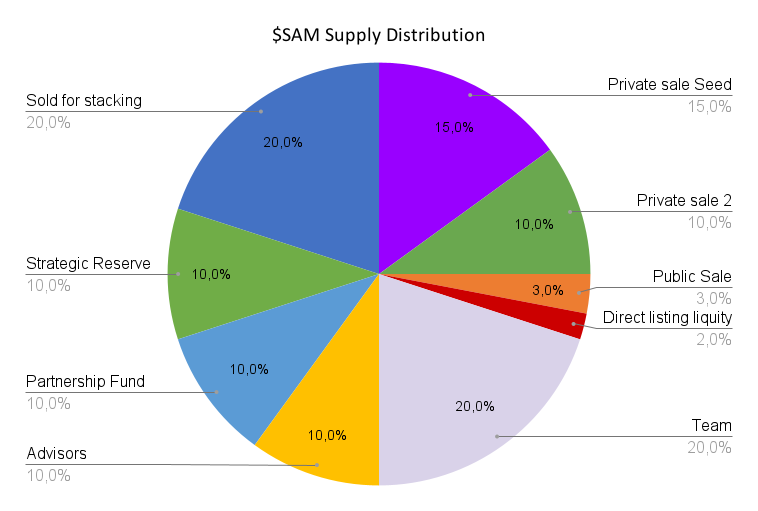
\includegraphics[scale=0.5]{SAM_Supply_Distribution.png}
\end{figure}

\begin{figure}[!h]
\centering
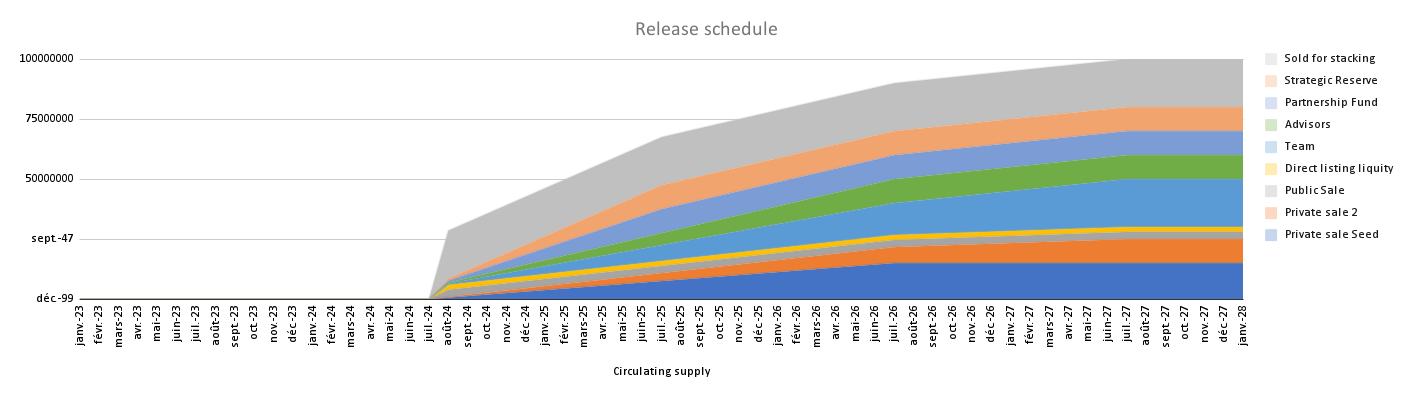
\includegraphics[scale=0.3]{Release_schedule.png}
\end{figure}

\newpage
\section{Clients}
\subsection{Produits Web3}
\begin{itemize} 
\item Bourses décentralisées \smallvspace
Les pools de liquidité sont des produits très répandus de DeFi. Des pools dédiés peuvent être très intéressants pour les institutions qui veulent acheter des cryptomonnaies pour leurs clients et eux-mêmes. Un pool ETH/USDC Certified Trust Space\texttrademark changerait la donne pour de nombreuses banques et fonds afin de réduire leurs risques d'être utilisés par des contre-parties malveillantes et d'assurer la conformité des fonds tout en protégeant le pseudonymat des participants. 

\item 
Launchpads \smallvspace
Les launchpads sont soumis à la pression des régulateurs en raison du volume de fonds qu'ils manipulent ; de nombreuses ICO ont été réalisées sans aucun contrôle KYC ou anti-blanchiment. De plus en plus, ces fournisseurs sont disposés à ajouter des contrôles KYC ou KYT à leurs plateformes. Nous allons créer des Certified Trust Spaces\texttrademark à l'intérieur des launchpads pour leur permettre d'être en conformité avec la réglementation anti-blanchiment. En n'acceptant que les portefeuilles homologués par Sesame, ces acteurs réduiront de manière significative le risque d'héberger des fonds douteux, allégeant ainsi le fardeau d'un cadre réglementaire toujours plus important et incitant des millions de nouveaux utilisateurs à rejoindre leur plateforme.

\item 
Fournisseur de portefeuilles crypto \smallvspace
Un fournisseur de portefeuille crypto ferait un parfait usage du Certified Trust Space\OldTexttrademark. En intégrant notre label et notre passeport sésame à l'embarquement, il réduira le risque de conformité pour l'entité à l'origine du service de portefeuille crypto et permettra la création d'une clientèle de premier ordre ne détenant que des jetons propres.

\item 
Blockchain proof of stake validator pools \smallvspace
À plus grande échelle, nous nous associons à des blockchains afin de garantir la conformité de tous les actifs mis en jeu pour le consensus de preuve d'enjeu. En scannant les portefeuilles et en aidant les nouveaux projets à créer un Certified Trust Space\OldTexttrademark, nous aidons les chaînes à attirer des institutions et des investisseurs individuels, ajoutant ainsi une nouvelle dimension à leur écosystème sans en diminuer la valeur ajoutée ou les principes fondamentaux.

\item 
Casinos et plateformes de paris \smallvspace
Plusieurs entreprises de premier plan préparent des systèmes de casino et de paris sportifs basés sur la blockchain. Mais les deux ont la réputation d’aider à blanchir de l'argent dans le monde physique ainsi qu'en ligne. En introduisant des Certified Trust Space\texttrademark au sein des plateformes de jeux, de paris et de jeux d'argent, nous pouvons imaginer une nouvelle façon pour les gens d'interagir en toute sécurité et pour que ces acteurs puissent intégrer des crypto-actifs de manière sûre et conforme.

\item 
NFTs Marketplace \smallvspace
À l'instar des casinos, l'art est parfois considéré comme un moyen de blanchir des profits douteux, et le problème se manifeste désormais sur les places de marché NFT. Grâce à notre solution, les maisons de vente aux enchères et les places de marché NFT peuvent créer une passerelle permettant uniquement aux détenteurs du certificat Sesame de participer à une vente en excluant les actifs numériques douteux Ainsi, nous réduisons considérablement le risque de blanchiment d'argent et créons un espace plus sûr pour l'art numérique.
\end{itemize}

\subsection{Institutions financières et prestataires de services financiers}
Se lancer dans l'espace crypto après des années dans un secteur donné est un défi de taille. Cependant, offrir des services crypto deviendra absolument nécessaire pour toutes les institutions financières dans les années à venir. En intégrant la solution Sesame KYT à ses procédures KYC et AML existantes, tout gestionnaire de patrimoine ou toute banque sera en mesure de servir une multitude de détenteurs de crypto-monnaies avec un risque minimal et un scoring individuel pour toutes leurs adresses. \\

Pour cette partie de la solution Sésame, nous offrons à la fois un scoring on-chain et off-chain, selon ce qui convient le mieux à l'institution financière partenaire.

\newpage
\section{Architecture Technique}
\subsection{Version 1.0 (2022)}
La première version de la solution comprendra une interface accessible en ligne par tous, où un utilisateur pourra payer pour tester son portefeuille et l’enregistrer dans la liste blanche, dans la mesure où le score agrégé de son portefeuille à partir des différents fournisseurs AML satisfait aux critères de conformité (par ceci on entend un score supérieur à un seuil défini par Sésame, en lien avec les réglementations et nos analyses statistiques).
La liste blanche est un smart contract on-chain géré par le propriétaire du contrat, ce qui signifie qu'un seul portefeuille est autorisé à y insérer ou supprimer des adresses. Un micro-service off-chain de gestion de la liste blanche est chargé de cette tâche pour le compte de l'interface d'enregistrement ou du programme de surveillance (voir Fig. 1).
Une copie de la liste blanche est stockée dans une base de données off-chain afin de conserver une sauvegarde des adresses de la liste blanche. Cette base de données off-chain répond également aux requêtes du service de surveillance afin de maintenir le programme de surveillance en synchronisation avec la création de nouveaux blocs dans la chaîne (dans l’état actuel des technologies, la réactivité d'une base de données centrale est notamment supérieure à celle du smart contract décentralisé). Des vérifications régulières seront effectuées pour s'assurer que les entrées de la base de données sont en cohérence avec les entrées de la liste blanche du smart contract. \\

\begin{figure}[!h]
\centering
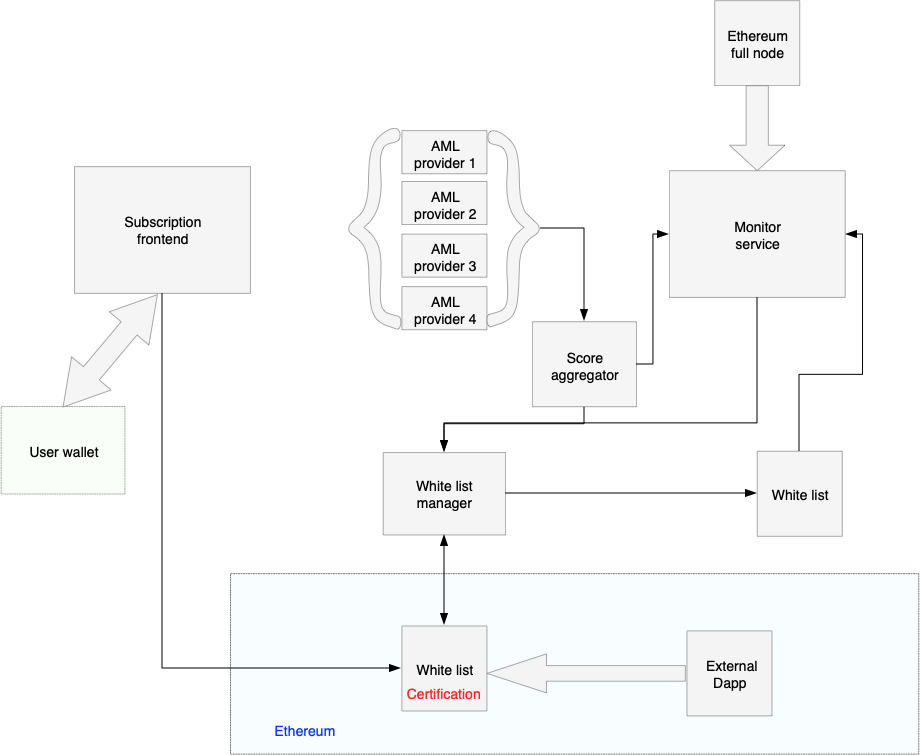
\includegraphics[scale=0.35]{architecture_v1_trim.png}
\caption{Architecture logicielle avec gestion de liste blanche off-chain}
\label{offchain}
\end{figure}


Le programme de surveillance vérifie chaque transaction de chaque bloc et identifie les adresses qui ont transféré des jetons vers les adresses de la liste blanche, ou par la suite celles auxquelles des tokens ont été envoyés. Si l'adresse de la contrepartie obtient un score suffisant, aucune modification n'est apportée à la liste blanche. En revanche, si l'adresse de la contrepartie n'est pas conforme, l'adresse de la liste blanche est re-testée, et si cette dernière interaction change son état de conformité, le programme de surveillance envoie une requête de publication au gestionnaire de la liste blanche pour supprimer l'adresse du destinataire de la liste blanche.
Une fois qu'une adresse a été enregistrée dans la liste blanche, le smart contract d’une application décentralisée tierce peut appeler une fonction du smart contrat de la liste blanche qui renverra une valeur booléenne "vrai" pour confirmer que l'adresse est bien conforme, et peut autoriser cette adresse à effectuer des transactions dans l’Espace de Confiance Certifié de l’application décentralisée.
Par souci de simplicité, dans un premier temps, la liste blanche ne sera valable que pour la blockchain où elle a été déployée puisque les applications décentralisées devront effectuer des appels de fonction au smart contrat de la liste blanche. Cependant, l'une des fonctionnalités à venir des partenaires AML est l'agrégation des scores de différentes blockchains compatibles EVM pour une même adresse. Cela signifie qu'un score sera identique pour une adresse donnée sur chaque chaîne où cette adresse possède des jetons. Une fois cette fonctionnalité opérationnelle, il sera techniquement possible pour les applications décentralisées d’effectuer des appels vers la liste blanche sur une blockchain et utiliser le résultat de conformité sur une autre blockchain de manière décentralisée grâce à l'utilisation d'une couche de transport de type PoS telle qu'Axelar Network (voir Figure 2). 
Cette dernière solution évitera les frais de gaz élevés liés à l'utilisation du réseau Ethereum. \\

\begin{figure}[!h]
\centering
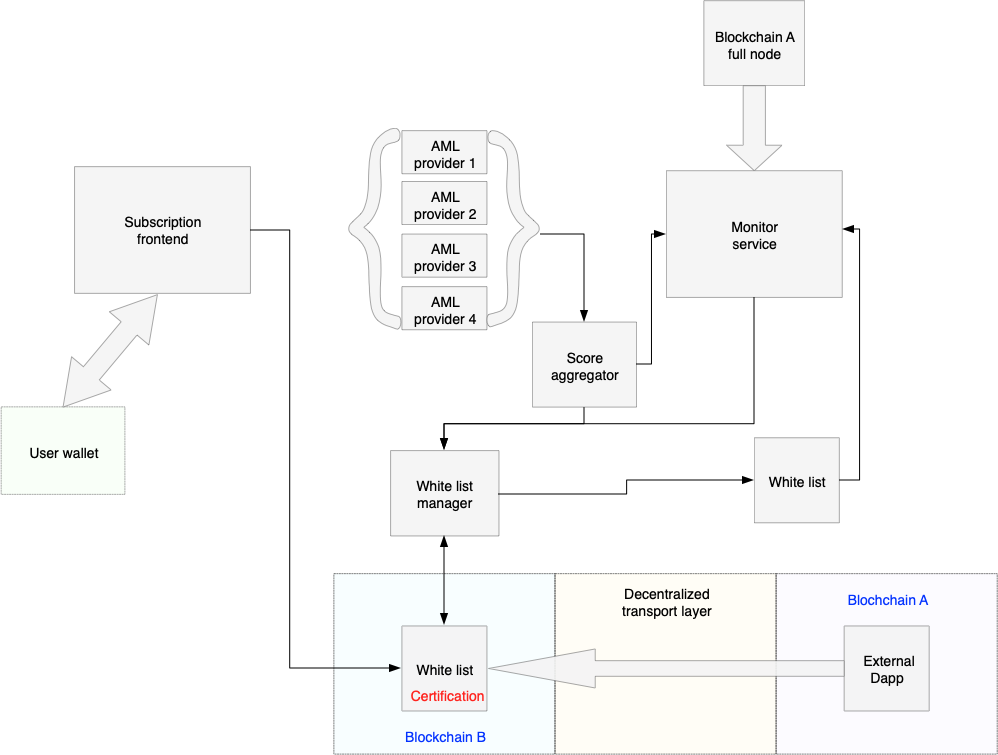
\includegraphics[scale=0.35]{architecture_v1_crosschain_trim.png}
\caption{Architecture logicielle avec gestion de liste blanche off-chain et fonctionnalité inter-chaînes}
\label{offchain}
\end{figure}  

Le statut de conformité est vérifié directement dans le smart contract du partenaire par un appel fonctionnel à la méthode de liste blanche déployée sur la blockchain. Le code en Solidity du smart contract, ses fichiers de déploiement JSON et ABI seront disponibles sur la page GitHub de Sesame. \\

Les partenaires qui souhaiteront accéder à la liste blanche à partir d'un appel de fonction on-chain à partir d'une chaîne différente de celle où la liste blanche a été déployée utiliseront la couche de transport pour acheminer l'appel de fonction d'une blockchain à l'autre.

\subsection{Version 2.0 (2023)}
La deuxième version de la solution utilisera un oracle pour amener la comparaison de notation d'adresse avec le seuil de conformité on-chain et augmentera donc la décentralisation et la transparence de la procédure de liste blanche (voir Fig. 2). Des fournisseurs Oracle tels que Chainlink ou API3 pourraient être utilisés pour effectuer cette tâche. \\

\begin{figure}[!h]
\centering
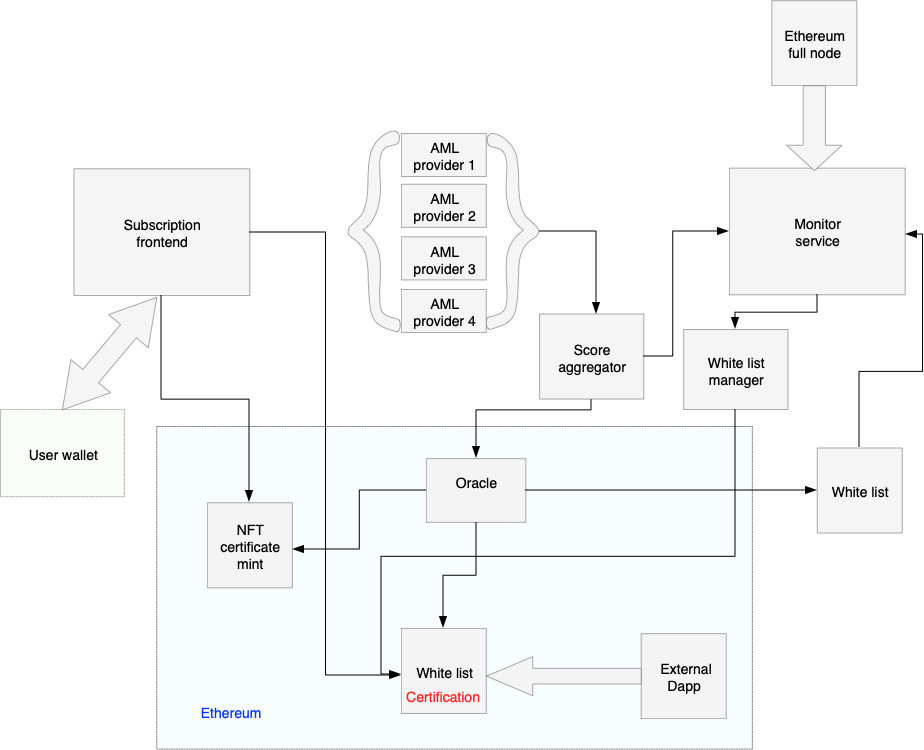
\includegraphics[scale=0.35]{architecture_v2_trim.png}
\caption{Architecture logicielle avec gestion de liste blanche on-chain et création de certificats NFT}
\label{onchain}
\end{figure}

À nouveau, une couche de transport, telle qu'Axelar Network, peut être utilisée pour héberger la liste blanche sur une chaîne et certifier les portefeuilles sur une autre (voir Figure 4).
Un oracle séparé, un pont NFT, ou une couche de transport pourront être aussi utilisés pour transférer le certificat vers une autre blockchain étant donné que le score du portefeuille, pour un portefeuille donné, a été agrégé à partir des données fournies par les partenaires AML. La technologie de liste blanche pourrait également évoluer vers un passeport NFT détenu par les utilisateurs conformes. \\
  
\begin{figure}[!h]
\centering
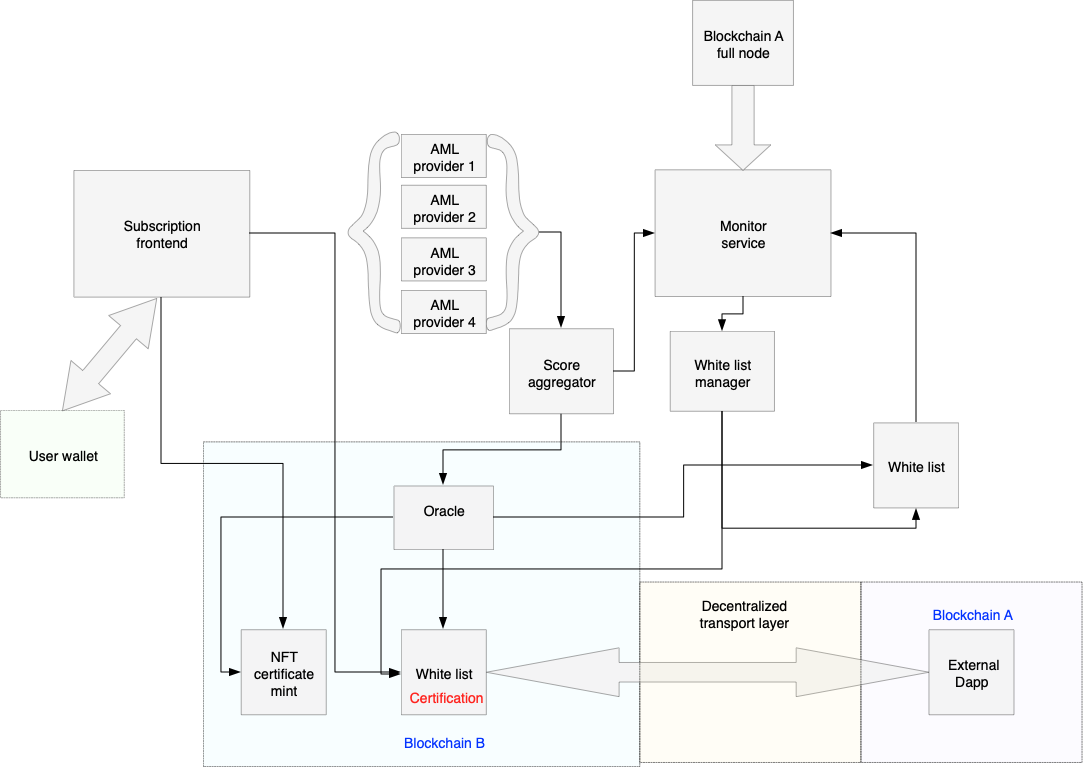
\includegraphics[scale=0.35]{architecture_v2_crosschain_trim.png}
\caption{Architecture logicielle avec gestion des listes blanches sur la chaîne et délivrance de certificats NFT avec fonctionnalité cross-chain}
\label{onchain}
\end{figure}


\subsection{Service de surveillance et suivi}
Le service de surveillance peut être exécuté directement sur un nœud complet Ethereum local afin de maximiser la vitesse de traitement de chaque transaction, en ne faisant pas de requêtes de procédure d'appel à distance (RPC) via Internet. Plusieurs nœuds peuvent être opérés simultanément pour optimiser les routes vers les différents fournisseurs AML.
A terme, le nombre de transactions dans un bloc peut devenir si important qu'une seule machine pourrait ne plus être en mesure de traiter toutes les transactions du bloc avant l'arrivée du bloc suivant. Dans ce cas, un traitement parallèle basé sur Apache Spark permettra aux demandes de vérification de transaction d'être adressées à un ou plusieurs nœuds.
Dans un modèle simplifié où les taux d'enregistrement et de désabonnement sont constants, si l'on considère également le pourcentage constant p de portefeuilles effectuant des transactions chaque jour parmi un nombre total de portefeuilles $\omega$ , le pourcentage de portefeuilles inscrits dans la liste blanche est donné par :

$$S(t)=1-\left(1-S_0\right)\mathrm{e}^{(c-r)t},$$

\noindent où $S_0$ est le pourcentage de portefeuilles pré-enregistrés sur la liste blanche au temps $t=0$, $0\le S(t)\le 1$~\footnote{L'\'evolution diff\'erentielle de $S(t)$ est intuitivement exprim\'ee par $\frac{\mathrm{d}S}{\mathrm{d}t}=(r-c)(1-S)$, et donne l'\'equation diff\'erentielle ordinaire $\frac{\mathrm{d}S}{\mathrm{d}t}+(r-c)S=r-c$.}.
Ensuite, le nombre d'adresses pour lesquelles le score est vérifié diminue avec le temps, tant que le taux de résiliation  est inférieur au taux d'enregistrement r, le nombre de transactions à suivre est :

$$\omega p\left[1-S(t)\right]=\omega p\left(1-S_0\right)\mathrm{e}^{(c-r)t}.$$

\subsection{Analyse statistique pour déterminer le  seuil de score de conformité}
Les fournisseurs AML utilisent différents systèmes pour noter les transactions qu'ils surveillent, et la plupart du temps, leur système est personnalisable par les utilisateurs de leurs solutions. Cela s'explique par le fait que les lois et réglementations varient d'un pays à l'autre. Par conséquent, il n'existe pas de norme internationale unifiée pour décider si un portefeuille doit être marqué comme conforme ou non.
Dans une première approche, Sésame visera à certifier les portefeuilles conformes au droit international communément connu, et choisira donc des paramètres qui reflètent cette internationalité.
Néanmoins, une comparaison statistique des résultats de notation des différents prestataires AML sera nécessaire afin de définir un seuil de score cohérent qui reflétera l'exigence des réglementations pour entrer dans l'Espace de Confiance Certifié\OldTexttrademark. L'équilibrage des scores de différents fournisseurs sera effectué sur la base d'une analyse statistique. Dans cette démonstration simplifiée, nous utilisons l'hypothèse que les portefeuilles sont uniformément répartis sur les solutions AML. L'ajustement peut se faire simplement en ré-alignant la moyenne et l'écart-type de la distribution des scores des différents prestataires AML avec un degré élevé de redondance.
Comme les scores sont tous compris entre 0 et 1 et tendent à être biaisés vers 1, on fait l'hypothèse que les scores fournis par chaque rapport AML suivent une distribution de Kumaraswamy, dont la fonction de densité de probabilité analytique est donnée par
$$P(x; a,b)=abx^{a-1}\left(1-x^a\right)^{b-a},$$  

\noindent où $a$ et $b$ ont des caractéristiques de paramètres de forme non négatifs caractéristiques au fournisseur AML.
Des méthodes de minimisation de type moindre carrés comme l'algorithme du gradient conjugué peuvent alors être utilisées pour ajuster les données collectées auprès des prestataires AML avec la distribution théorique P(x; a,b) afin que les paramètres a et b puissent être évalués.
Les dérivées utilisées pour le vecteur gradient sont$$\frac{\partial P}{\partial a}=\frac{bx^{a-1}\left(1-x^a\right)^{b-1}\left[a\ln(x)x^ab
-a\ln(x)+x^a-1\right]}{x^a-1}$$
et 
$$\frac{\partial P}{\partial b}=ax^{a-1}\left(1-x^a\right)^{b-1}\left[b\ln(1-x^a)+1\right].$$

Pour un certain nombre de fournisseurs AML, les paramètres de forme agrégés sont alors donnés par la moyenne des paramètres de forme individuels :
$$a=\sum_{i=0}^na_i$$
$$b=\sum_{i=0}^nb_i$$  

À l'avenir, l'outil pourrait être adapté aux réglementations locales du pays de manière à ce que l'utilisateur puisse choisir librement la juridiction à laquelle son portefeuille se conforme.

\subsection{Développements futurs : des passeports NFT aux chaînes de blocs privées}
\subsubsection{Confidentialité}
La confidentialité du certificat pourrait également être préservée en utilisant des preuves à connaissance nulle afin que le statut de conformité ne soit connu que de l'utilisateur et de la partie à laquelle il s'engage à la divulguer, c'est-à-dire les partenaires Web3 fournissant un Espace de Confiance Certifié. La preuve à connaissance nulle peut être mise en œuvre pour les contrats intelligents compatibles EVM à l'aide de la famille d'algorithmes zk-SNARKs et de la courbe elliptique alt\_bn128 qui font partie de EIP-196 et EIP-197. Dans ce cas, l'adresse du portefeuille et son score peuvent être chiffrés à l’aide des clés de vérification et stockés on-chain tandis que les clés de preuve peuvent être conservées par l'utilisateur.
Étant donné que le coût d'enregistrement des points de courbe elliptique sur la chaîne sera beaucoup plus élevé qu'une simple adresse de portefeuille ordinaire, la liste blanche cryptée pourrait être déployée sur une blockchain moins onéreuse, telle que Milkomeda Cardano, ou même un sous-réseau Avalanche dédié, de sorte que les frais de gaz seront proches de zéro.
Le cas d'un test d'acceptation décentralisé combiné à la confidentialité des scores pourrait également justifier la nécessité d'exécuter une blockchain privée où l'agrégation réelle des scores pourrait avoir lieu.

\subsubsection{Attestation sous forme de passeport}
Le certificat pourrait prendre la forme d'un passeport représenté par un NFT non transférable ou Soul Bound Token (SBT). La création d'un standard pour les SBT est attendue d’ici fin 2022, il sera donc envisageable de les intégrer dans la version 2.0 de notre solution prévue en 2023.
De plus, l’utilisation des SBT permettra le transfert des certificats d'une chaîne à l'autre. La technologie n'est pas encore complètement prête au moment de la rédaction, mais on peut déjà envisager l'utilisation de telles solutions pour diffuser la certification enregistrée dans une liste blanche unique à des applications sur de nombreuses blockchains. Cela simplifiera grandement la maintenance et la cohérence de notre produit.

\subsection{Appels à la liste blanche par les partenaires Web3}
La conformité d’une adresse est vérifiée dans le smart contract du partenaire ou sur son site Web par un appel fonctionnel à la méthode de liste blanche qui a été implémentée dans un smart contrat écrit dans Solidity. Le code du smart contract et son fichier de déploiement JSON seront disponibles sur le github Sésame.
Les partenaires qui souhaitent accéder à la liste blanche depuis un appel de fonction on-chain depuis une chaîne différente de celle où la liste blanche a été déployée utiliseront un oracle qui fera un appel à une API fournie par un service Sesame.
Dans le cas d'une liste blanche cryptée, l'état de conformité est vérifié de la même manière.

\newpage
\section{Feuille de route du produit, de l’entreprise Sésame et du jeton }

\begin{itemize}
\item
Q3 2022:  v0.1 POC
    \begin{itemize}
    \item Testnets compatibles EVM (Kovan, Rinkeby, local, Polygon PoS Mumbai, Avalanche C-Chain Fuji, Milkomeda Cardano, Binance Smart Chain). 
    \item Programme de surveillance en série. 
    \end{itemize}

\item
Q4 2022: v0.2 MVP
    \begin{itemize}
    \item Lancement du produit bêta privé sur testnet et mainnet.
    \item Accepter les paiements d'Ethereum, Binance Smart Chain, Avalanche C-Chain, Polygon PoS, Cronos, Fantom, Arbitrum, Milkomeda, Kava, Aurora, Optimism, Gnosis. 
    \item Scoring public gratuit des adresses compatibles EVM et enregistrement dans la base de données centrale.
    \item Programme de surveillance parallèle pour les r\'eseaux de test Ethereum sur Spark/Kubernetes.
    \item Audit.
    \end{itemize}

\item
Q1 2023: v1.0
    \begin{itemize}
    \item Lancement officiel d'une liste blanche on-chain et d'un moniteur pour le réseau principal Ethereum.
    \item Enregistrement on-chain des adresses à partir de la base de données centrale.
    \item Produit sans staking. Tout utilisateur supprimé de la liste blanche doit se réabonner.
    \item Utilisation d'Axelar Network et d'oracle sur des réseaux de test compatibles EVM (Ropsten, Polygon PoS Mumbai, Avalanche C-Chain Fuji).
    \end{itemize}

\item
Q2 2023: v1.1
    \begin{itemize}
    \item Lancement officiel d'une liste blanche sur la chaîne et d'un moniteur pour Binance Smart Chain et Polygon PoS.
    \item Utilisation de zk-SNARKs sur des réseaux de test compatibles EVM (Avalanche C-Chain Fuji, etc). 
    \end{itemize}

\item
Q3 2023: v2.0
    \begin{itemize}
    \item Utilisation d'Axelar Network pour le calcul d’inscription en chaîne de nouveaux portefeuilles sur Ethereum, Binance Smart Chain, Polygon PoS.
    \item Migration de la liste blanche Avalanche C-chain
    \item Frappe du jeton SAM sur Avalanche C-Chain.
    \end{itemize}

\item
Q4 2023: v2.1
    \begin{itemize}
    \item Mise en place d'un pool de liquidités et de stacking. 
    \item Lancement officiel d'une liste blanche pour Tron.
    \item Introduction en bourse du jeton.
    \end{itemize}

Le gestionnaire de liste blanche vérifie l'adresse des jetons SAM investis dans le pool de liquidité afin de vérifier si les jetons requis sont présents.

\item
Q1 2024 v2.2
    \begin{itemize}
    \item Lancement officiel d'une liste blanche publique et d'un moniteur pour le réseau Avalanche C-Chain.
    \item D\'ebut de l'adaptation aux chaînes non EVM : Stacks, Ripple, Cosmos, Solana.
    \end{itemize}

\item
Q2 2024 v2.3
    \begin{itemize}
    \item Lancement officiel d'une liste blanche et d’un programme de surveillance pour Stacks, Ripple, Cosmos, and Solana.
    \end{itemize}
\end{itemize}

\newpage
\section{Remarques finales}

Le portefeuille crypto et la certification du projet Web3 ne sont que les premières étapes pour Sésame. La certification en tant que modèle commercial peut être déclinée en une myriade de secteurs d'activité et de diverses industries en capitalisant sur les caractéristiques uniques de la technologie blockchain et les innovations cryptographiques.
La certification peut être appliquée à des considérations environnementales, sociales ou financières ainsi qu'au respect d'un ensemble d'autres critères spécifiques, tels que ceux basés sur des principes de communauté. L'utilisation de la blockchain conduira à un espace numérique plus transparent et sécurisé grâce à l'utilisation de plateformes de certification décentralisées pour les chaînes de blocs, et à la capacité de chaque utilisateur à utiliser et bénéficier de cette technologie révolutionnaire. \\

{\bf Rejoignez-nous maintenant !}

\newpage
\section{Avertissement Légal} 
(cf. version EN)

\end{document}
